\documentclass[11pt]{beamer}
\usetheme{Boadilla}

\usepackage[utf8]{inputenc}
\usepackage[T1]{fontenc}
\usepackage{amsmath}
\usepackage{amsfonts}
\usepackage{amssymb}
\usepackage{graphicx}
\usepackage[scaled=0.85]{beramono}
\usepackage{listings}
\lstset{language=C++,
	columns=fullflexible,
	basicstyle=\ttfamily,
	tabsize=4,
} 
\usepackage[english]{babel}

\graphicspath{
	{\string~/Code/networkit/egosplit/plots/}
}


\begin{document}
	\author{Armin Wiebigke}
	\title{Ego-Splitting Framework}
	%\subtitle{}
	%\logo{}
	%\institute{}
	%\date{}
	%\subject{}
	%\setbeamercovered{transparent}
	%\setbeamertemplate{navigation symbols}{}
	\begin{frame}[plain]
	\maketitle
\end{frame}

\begin{frame}{Idea}
\begin{itemize}
	\item Problem: Overlapping community detection
	%\item Each node can be part of multiple communities
	\item Reduce problem to non-overlapping communities (partition)
	\begin{itemize}
		\item Many established algorithms
	\end{itemize}
	\item Two partition algorithms: local and global
	\item \emph{Ego-net} of node \textit{u}: Subgraph induced by the neighbors of \textit{u}
\end{itemize}
\end{frame}


\begin{frame}{The Framework}
\begin{itemize}
	 \item For each node:
	 \begin{itemize}
	 	\item Create the ego-net graph (triangle search)
	 	\item Use the local clustering algorithm to partition the ego-net
	 \end{itemize}
	 \item Create persona graph:
	 \begin{itemize}
	 	\item Create a persona for each partition
	 	\item Add edges between personas
	 \end{itemize}
\end{itemize}
\vfill
\centering
\includegraphics[height=65pt]{/home/armin/Documents/create_persona.pdf}
\end{frame}

\begin{frame}{The Framework}
	
\begin{itemize}	
	\item Use the global clustering algorithm on the persona graph
	\begin{itemize}
		\item Each partition is one community
	\end{itemize}
	\item For each node: Collect communities from all personas
	\end{itemize}
	\vfill
	\centering
	\includegraphics[height=85pt]{/home/armin/Documents/partition_persona.pdf}
\end{frame}

\begin{frame}{Problems}
	\begin{itemize}
		\item Local partitioning is critical
		\begin{itemize}
			\item number of Communities $\leq$ number of Personas
			\item Detecting communities in ego-net can be difficult/impossible
			\item Repairing possible?
		\end{itemize}
%		\item Triangle with two nodes in community and one outside $\Rightarrow$ outside node is included in community by global partition algorithm 
	\end{itemize}
\end{frame}

\begin{frame}{Problems}
	\begin{itemize}
		\item Which partition algorithm(s)?
	\end{itemize}
	\centering
	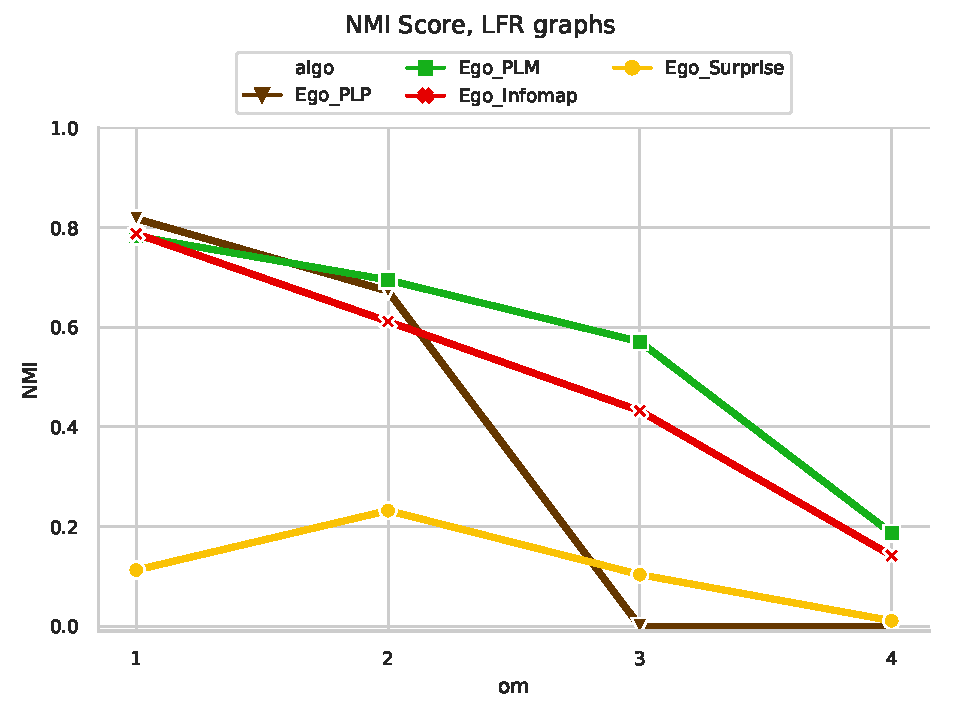
\includegraphics[width=0.8\linewidth]{metrics/NMI_score_LFR_om_ego.pdf}
\end{frame}


\begin{frame}{Possible Improvements}
	\begin{itemize}
		\item Clean-up at the end (OSLOM)
	\end{itemize}
	\centering
	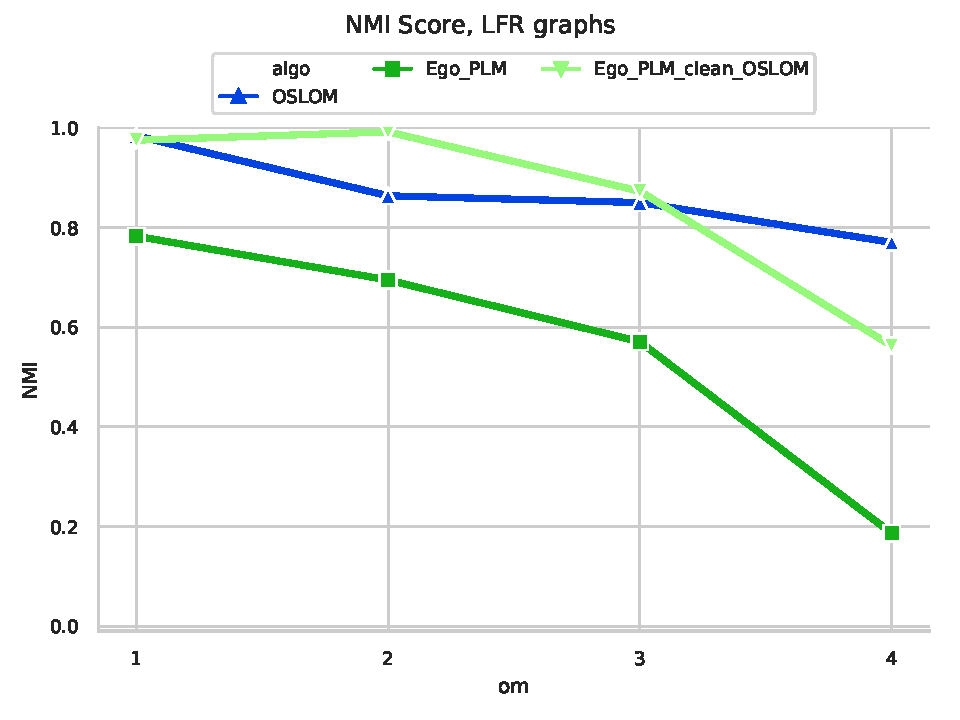
\includegraphics[width=0.8\linewidth]{metrics/NMI_score_LFR_om_clean.pdf}
\end{frame}

\begin{frame}{Possible Improvements}
	\begin{itemize}
		\item Connect personas of one node with additional edges
		\item Combinations of local/global algorithms
		\item Increase size of ego-net
		\begin{itemize}
			\item neighbors of neighbors
			\item squares
		\end{itemize}
	\end{itemize}
\end{frame}

\begin{frame}{Plots}
\centering
\includegraphics<1>[width=0.8\linewidth]{metrics/time_LFR_om_clean.pdf}
\includegraphics<2>[width=0.8\linewidth]{communities/comm_sizes_LFR_om_3.pdf}
\end{frame}
\end{document}